% This is samplepaper.tex, a sample chapter demonstrating the
% LLNCS macro package for Springer Computer Science proceedings;
% Version 2.21 of 2022/01/12
%
\documentclass[runningheads]{llncs}
%
\usepackage[T1]{fontenc}
% T1 fonts will be used to generate the final print and online PDFs,
% so please use T1 fonts in your manuscript whenever possible.
% Other font encondings may result in incorrect characters.
%
\usepackage{graphicx}
\graphicspath{{./pics/}}
% Used for displaying a sample figure. If possible, figure files should
% be included in EPS format.
%
% If you use the hyperref package, please uncomment the following two lines
% to display URLs in blue roman font according to Springer's eBook style:
%\usepackage{color}
%\renewcommand\UrlFont{\color{blue}\rmfamily}
%\urlstyle{rm}
%
\usepackage{xurl}
\usepackage{amsfonts}
\usepackage{amssymb}
\usepackage{amsmath}
\usepackage{listings}
\setcounter{secnumdepth}{4}

\begin{document}
%
\title{Visualization of LLL and BKZ Algorithms with Vector Representations}
%
%\titlerunning{Abbreviated paper title}
% If the paper title is too long for the running head, you can set
% an abbreviated paper title here
%
%\author{Muhammad Imam Chaidar Mujaddid Al-Ghiffari\inst{1}\orcidID{0000-1111-2222-3333} \and
%Amril Syalim \inst{2,3}\orcidID{1111-2222-3333-4444}}
\author{Muhammad Imam Chaidar Mujaddid Al-Ghiffari \and Amril Syalim}
%
\authorrunning{Muhammad Imam Chaidar Mujaddid Al-Ghiffari et al.}
% First names are abbreviated in the running head.
% If there are more than two authors, 'et al.' is used.
%
\institute{Faculty of Computer Science, Universitas Indonesia}

%\email{https://cs.ui.ac.id/}
%
\maketitle              % typeset the header of the contribution
%
\begin{abstract}

As the quantum computing starts to threaten the current cryptographic systems such as RSA, cryptographers around the world start to develop the Post-Quantum Cryptography (PQC) algorithms, most of them are lattice-based (for example ML-KEM and ML-DSA), which are strong enough to withstand attacks from quantum-based cryptanalysis techniques such as Shor's algorithm, Grover's algorithm, and other quantum cryptanalysis algorithms. In order to strengthen these PQC algorithms, cryptographers and cryptanalysts alike also developing LLL and BKZ algorithms to test the strength of these PQC algorithm. One of the problems with LLL and BKZ is the fact that while these algorithms are able to penetrate PQC systems, they're harder to learn compared to the algorithms which they succedeed. Sufficient mathematical understanding is required in order to get proper understanding of these algorithms. Some online tools have been available, especially for LLL algorithm, in order to visualize these algorithms so learners can learn them easier. The problem is that many of these visualizations only show the initial and the final result of the input. In this paper, we will build a tool to visualize the processes of both LLL and BKZ algorithms. Through visualization with vectors on Cartesian coordinate as well some panels such as Lovasz status panel and other panels that will explain the current stage of the process of both LLL and BKZ, we expect cryptography learners and enthusiasts alike to understand LLL and BKZ easier. 

\keywords{Cryptography  \and Cryptanalysis \and Post-Quantum \and Lattice \and LLL \and BKZ.}
\end{abstract}
%
%
%
\section{Introduction}

Cryptanalysis is the technique of analysing and breaking a ciphertext to obtain the plaintext (A. Al-Sabaawi, 2020). The history and the development of cryptanalysis itself can't be separated from the history and development of cryptography. With the onset of the development of quantum computing and subsequently quantum cryptanalysis, many commonly used modern cryptographic algorithms, especially RSA, are threatened by quantum cryptanalysis (). Which is why cryptographers around the world already started to develop cryptographic algorithms that can resist quantum cryptanalysis - the post-quantum cryptography (PQC) (). Most of PQC algorithms that are seen as promising, are lattice-based (Shaik Ahmadunnisa et al, 2025). For example, Kyber and Dilithium and their standardized versions - the ML-KEM and ML-DSA algorithms. At the same time, cryptanalysts and cryptographers also use these lattice reduction cryptanalysis algorithms in order to evaluate the strength of these lattice-based PQC algorithms to resist their greatest foe - none other than the lattice reduction cryptanalysis algorithms ().

The most common lattice reduction technique is the LLL algorithm, which was already developed long before the advent of quantum computing, and obviously predates the PQC algorithms as well. A polynomial-time algorithm for finding a short and nearly orthogonal basis for a lattice, this algorithm can be used to solve the shortest vector problem (SVP) and the closest vector problem (CVP), which are essential in lattice-based cryptography. We could say that LLL is the foundation of the lattice reduction cryptanalysis algorithms, and to master the subsequent algorithms, mastering the LLL before is a crucial step. 

For now, the most promising lattice-based cryptanalysis technique is the BKZ algorithm, which is basically the upscaled version of the LLL algorithm (). Compared to LLL, BKZ can find even shorter vectors in a lattice () and theoritically speaking, BKZ is a far greater threat to lattice-based PQC systems compared to LLL, which are no longer a major threat for these lattice-based PQC systems. To help learners learn LLL and BKZ algorithms, some online solver tools have been developed, for example fplll and fpylll, Sage Cell, and lll-attack-runner. 

The problems with these LLL and BKZ solvers is that they are either only show the final result, less user-friendly compared to simpler matrix tools, doesn't have visualization, or doesn't show the mathematical processes between the initial state and the final result. The first problem is true for fplll, fpylll and lll-attack-runner, as they only show the final result. The second problem is true for Sage Cell, as we can't just insert a "plain" matrix to process it, we have to wrap the matrix within either a Python code, a Sage code, or any code in at least one of languages available in the tool. To put it simply, it isn't as practical as inserting the matrix in some simpler online matrix tools, such as Calculator.net, matrixcalc.org, or Desmos. And the third problem is true for fplll and fpylll as well Sage Cell, as they don't even have built-in visualization. Sage Cell can show every step of the LLL process, however, we need to modify the code we inserted in the tool, in a manual way, so we can't use the built-in method of .lll(), and we have to use our own code. For the fourth problem, all previously mentioned LLL and BKZ algorithms solvers have this problem. None of these solvers show the mathematical processes between the initial state and the final result. For Sage Cell, there is no built-in library to show these steps.

So in short, these LLL and BKZ tools aren't practical compared to several online math tools, and they don't automatically provide visualization from the beginning to the final result nor that they provide the step-by-step explanation. Which is actually an important issue, because psychologically wise, humans are generally easier to process information visually (Mayer, 2001) but also how the users interact with them is also an important factor (Christopher D. Hundhausen et al, 2002). So we definitely need step-by-step explanations just like we need the visualizations, within a system that lets the user to interact with the system from the input insertion to the output visualization. For the visualization part, it's clear that visualization through vectors can significantly help users to understand the process. Why? Because the basis concept for LLL and BKZ is lattice reduction. Which is a linear algebra concept. And it is hard to teach the concepts of linear algebra without vectors (or, to be more precise, vector geometry) visualization (Konyaliouglu et al., 2011). 

Our idea is that by visualizing LLL and BKZ algorithms from the beginning of the process until the final result with vectors on 2D and 3D Cartesian coordinates, showing the calculations behind the algorithms, as well some simple theoritical explanations of these algorithms, we can help the users to understand these algorithms easier. The inputs are in the form of matrices. We will develop a tool that not just process LLL and BKZ algorithms, but also show the visualization from the initial state until the final result, with simplified processes shown to help users understand these two algorithms easier. Our main idea for the visualization is through the usage of vectors within a Cartesian field, both in 2D and 3D projections, as well several panels that showing the current process (and its explanation), Lovasz condition status, and a button that can be pressed to go to the previous and next steps. We hope that through these visualization and textual elements, users would have it easier to understand the mechanism of both LLL and BKZ algorithms, which are increasingly becomes more relevant for the security of our data.


\section{Related Works}
\subsection{Learning with Errors(LWE)}
\mbox{}
Learning with Errors (often shortened to LWE) is very essential for modern lattice-based PQC algorithms, such as NIST's ML-KEM and ML-DSA (Wang et al., 2025). Basically, this is a method to hide the information (e.g plaintext) by injecting randomized noises (errors) into a system of linear equations which represents the public matrix, which would make the attackers struggling to get the actual pieces of the information from the plaintext. To solve an LWE problem means solving a set of linear equations with errors hidden in the equations. The errors are often tiny. 

For example, there is a public matrix $A$, our secret message or plaintext $s$, and a random small number to mess the equation $e$. Normally, without the latter, a cipher is usually defined as $C = As \pmod q$. With LWE however, the equation becomes $C = As + e \pmod q$. Without the small errors, we can solve the system of linear equations with Gaussian Elimination, and thus the encryption algorithm is easier to cracked. 

There are two types of LWE : 
\begin{itemize}
\raggedright
\item Search LWE. This approach is to find $s$ - the secret key from a noisy set of linear equations. 

\item Decision LWE. This approach is to distinguish an equation with LWE from a pure random noise. Usually, a real LWE set of equations would actually at first look random, but the errors gained from the solutions (gained from lattice reduction algorithms, not Gaussian elimination) of these equations do usually cluster around the actual key. 
\end{itemize}

As the best practice, the size of the randomized error must small enough to make it decipherable for the intended receivers of the encrypted data. Small errors also able to force the attackers to switch into lattice reduction problem (because the errors resulted from attempts to solve these linear equations using Gaussian elimination), which essentially the same as searching shortest vectors (the SVP problem). Which, of course forcing the attackers to convert the system of linear equations into a lattice. 

\subsection{Lattice}
\mbox{}
A lattice is defined as a set which contains every single linear combinations of vectors from a basis of $\mathbb{R}^n$. Therefore, we can state that a lattice is theoritically a discrete subset of vector space with the dimension size of $n$. 

Let's say, we have $L$, which is a lattice, then :
\begin{itemize}
\raggedright
\item $k$ is the rank or the dimension size of $L$
\item ${\{v_1, v_2, ....v_k\}}$ is the basis of $L$.
\end{itemize}

$L$ must have vectors of $v_1, v_2, .....v_k$ that each of these vectors are linearly independent and such that $L = \mathbb{Z}$-linear span of ${\{v_1, v_2, ....v_k\}}$ (Silverman H. Joseph, 2020).

Lattice is one of the key mathematic concepts of the Post-Quantum Cryptography, in fact, of the four PQC algorithms that have been selected by NIST in order to be standardized, three are based on lattice : ML-KEM (based on CRYSTALS-Kyber), ML-DSA (based on CRYSTALS-Dilithium), and FN-DSA (based on Falcon). 

\subsection{Lattice-based Post-Quantum Cryptography}
\mbox{}
The lattice-based PQC is a group of cryptographic algorithms that like its name, are based on lattices, and their security is dependent on the hardness on two computational problems that are considered hard even for quantum cryptanalysis algorithms (such as Shor's Algorithm) to solve in the polynomial time : Shortest Vector Problem (SVP) and the Closest Vector Problem (CVP). Example for lattice-based PQC algorithms are : 
\begin{itemize}
\raggedright
\item CRYSTALS-Kyber. Standardized by NIST into ML-KEM (Module Lattice-based Key Encapsulation Mechanism). This algorithm, just like its pre-standardized version, is a set of algorithms used for two parties in order to establish a shared secret key in a channel considered to be unsafe.
\item 
\item CRYSTALS-Dilithium. Standardized by NIST into ML-DSA (Module Lattice-based Digital Signature Algorithm). It is a set of algorithms that is used to generate as well verify digital signatures.
\item
\item Falcon (Fast Fourier Lattice-based Compact Signatures Over NTRU). Standardized by NIST into FN-DSA. It's also a DSA like ML-DSA. 
\end{itemize}

Because most lattice-based PQC are using LWE to make their linear equation systems noisier, the problem essentially becomes equivalent (or at least related) to finding unusually short vectors, finding close lattice points, or reducing the lattice basis into a more orthogonal form. This is how the lattice basis reduction plays a vital role - although it doesn't guarantee the lattice-based PQC algorithm to be cracked. 

\subsection{Lattice Reduction}
\mbox{}

Lattice reduction is a process to find shortest vectors or closest vectors in lattices (Silverman H. Joseph, 2020). Within a lattice reduction process, the bases considered to be "bad," highly non-orthogonal basis (where the vectors are long and meet at sharp angles) are transformed it into a better version of them, which are reasonably orthogonal (each of their respective vectors are perpendicular to each other, vectors meet at angles closer to 90 degrees, and are relatively short). Why do we need "good" bases? Because good bases make hard lattice problems computationally easier to be solved. 

Hadamard's Inequality is a method to tell a basis is a good or bad one. 

\begin{equation}
Det(L) \leq \Vert v1 \Vert . \Vert v2 \Vert .... \Vert vn \Vert
\end{equation}

This inequality clearly states that the determinant of a lattice is always less than or equal to the product of the lengths of its basis vectors. For a bad basis, the product of the vector lengths is drastically larger than the true determinant (the determinant of the lattice where the basis belongs to). For a good basis, the product of the vector lengths are very close to the true determinant of the lattice. A "perfect" basis essentially has the same product of vector lengths with their true determinant. To put it simple, the closer the product of the vector lengths of a basis to the value of its true determinant, the better the basis is. 

So, with lattice reduction, we can pick any single bad basis and turn it into a better version of it. 

The most known modern lattice reduction method is Lenstra-Lenstra-Lovasz lattice reduction algorithm, often shortened to LLL. Virtually all modern mainstream lattice reduction algorithms are based on the LLL framework. For example, the Block Korkine Zolotarev (BKZ) lattice reduction algorithm uses LLL as an important kind of steps of it. 

\subsection{Shortest Vector Problem}

The SVP (Shortest Vector Problem), like its namesake, is the problem of finding a shortest and non-zero vector in a lattice (Silverman H. Joseph, 2020). For a vector in a lattice to be regarded as the SVP, a vector must be the shortest one (or the shortest ones), out of all vectors in the lattice, and it must be a nonzero vector. 

SVP is essential for PQC lattice reduction algorithms because it can help to solve the hidden noises injected in linear equations (the LWE problem) used in PQC algorithms. 

\subsection{LLL}
\begin{figure}[htbp]
    \centering
    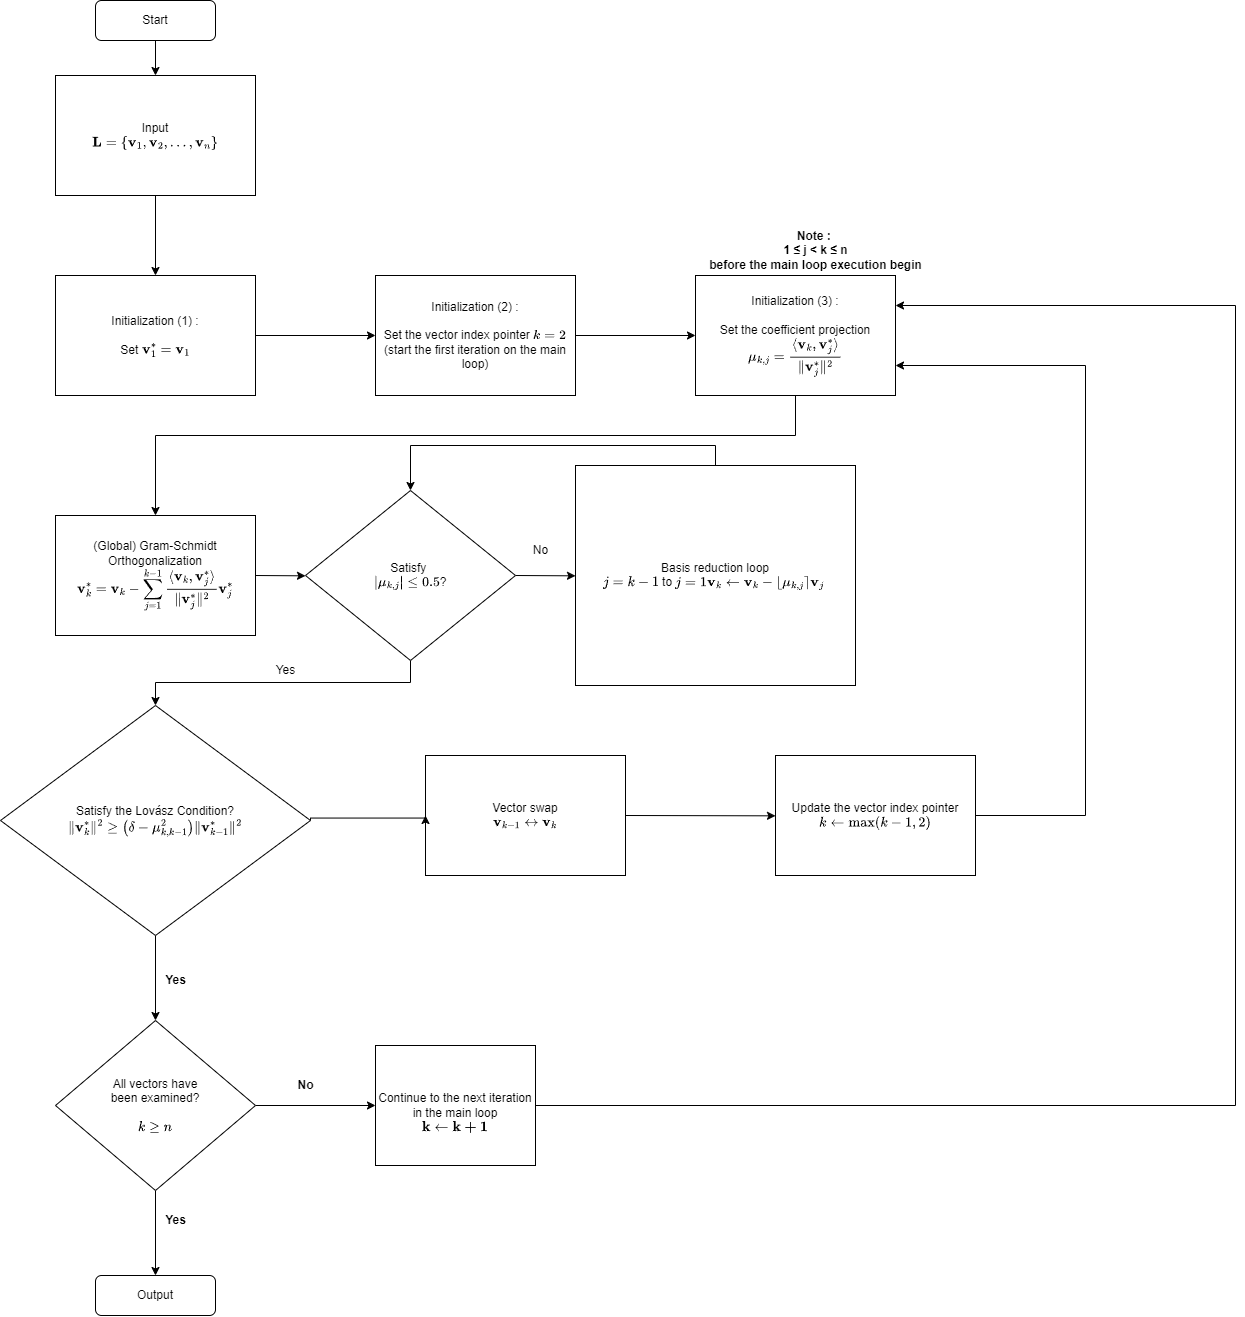
\includegraphics[width=0.7\textwidth]{lllrevisi.png}
    \caption{The LLL algorithm}
    \label{LLL}
\end{figure}
\mbox{}

[to do : correct the diagram and add more explanations]
[to do : add pseudocode]
The LLL (Lenstra-Lenstra-Lovasz) cryptanalysis algorithm, developed by Arjen Lenstra, Hendrik Lenstra, and Laszlo Lovasz in 1982, is a lattice reduction algorithm. Although LLL in present days is largely ineffective to reduce lattices in many PQC algorithms such as ML-KEM and ML-DSA, the LLL is the foundation of modern lattice reduction cryptanalysis. For example, it serves as the foundation of BKZ, the upscaled version of LLL, by having several LLLs processes executed for a single BKZ process. 

In the Fig.1, we can see how the algorithm works. The usual inputs are in the form of matrices, or a set linear equations. Either way, the acceptable form of input in our tool is matrix. However, in the general context, for a single LLL process, the input is in the form of a lattice basis $L$, which are in the form of a set of basis vectors ${\{v_1, v_2, ....v_n\}}$. Later for every vector within the set, they will be iteratively processed by Gram-Schmidt orthogonalization, then reduction or swap, and then examined whether the basis at the index fulfills the Lovasz Condition or not. The iteration process, however, is controlled by a pointer variable $k$ which starts from 2nd index to the $n$-th index (the last vector). In other words, the first vector only acts as a projection reference for Gram-Schmidt orthogonalization (it only acts as the initial orthogonal basis ($\mathbf{v}_1^* = \mathbf{v}_1$)) and size reduction processes of subsequent vectors, but the first vector is never individually subjected to the vector swap mechanism (unless during the first iteration, the second vector fails to meet the Lovász Condition checking) or Lovász Condition checking. After all subsequent vectors have gone through these processes, the loop ends and the algorithm stops. 

Unless the initial lattice basis is already a highly orthogonal basis, we will obtain a more orthogonalized and shorter version of the basis. Thus, with a basis that is more orthogonal and shorter, we would have it easier for recovering the LWE small errors hidden in the linear equations that form the public matrix we want to crack. 

As an important note, the $\delta$ value used in Lovász Condition ranges from 0.25 as the minimum value to 0.99 as the maximum value. A higher $\delta$ yields higher quality outputs at the expense of more iterations, and a lower $\delta$ leads to fewer iterations at the expense of lower quality outputs. In other words, a higher $\delta$ makes the recovery of the LWE errors easier.

\subsubsection{Initialization}
\mbox{}
$$\mathbf{L} = \{v_1, v_2, ....v_n\}$$
We have $L$, a lattice basis, with $n$ vectors within it. The $L$ contains ${\{v_1, v_2, ....v_n\}}$. Assume $L$ is a "bad" basis, then our goal is to make it more orthogonal and shorter. 

\subsubsection{Gram-Schmidt orthogonalization}
\mbox{}
$$\mathbf{v}_k^* = \mathbf{v}_k - \sum_{j=1}^{k-1} \frac{\langle \mathbf{v}_k, \mathbf{v}_j^* \rangle}{\|\mathbf{v}_j^*\|^2} \mathbf{v}_j^*$$

Right after the initialization, the algorithm processes the basis vectors sequentially. At the global scale (or the outer loop) in $L$, the algorithm performs Gram-Schmidt orthogonalization (GSO) for all vectors in $L$, produces the initial orthogonalized $\mathbf{v}_k^*$ and their corresponding projection coefficients $\mu_{k,j}$, with $1 \le j < k \le n$ before the main loop execution begins. Notice that for the first vector ($k = 1$), no projection is needed since it has no preceding vectors. Hence, $\mathbf{v}_1^* = \mathbf{v}_1$.

\subsubsection{Main loop}
\mbox{}
After the global Gram-Schmidt orthogonalization process, the index pointer $k$ points at the second vector from the left (the vector of $v_2$), thus the main loop begins with the first iteration begins at $k=2$.

\subsubsection{Basis reduction loop}
\mbox{}
The algorithm checks the size of the vector, and then performs a size reduction of the vector to ensure that the length of the projection coefficients satisfies : $$|\mu_{k,j}| \leq 0.5$$ To satisfy the condition, the algorithm uses an internal index pointer, $j$, whose sole purpose is to become the backward iterator in this basis reduction loop, and this loop starts from $j = k - 1$ down to $1$. This ensures that the current target vector $\mathbf{v}_k$ is systematically reduced against all of its preceding vectors in the basis. The vector $\mathbf{v}_k$ is then iteratively updated using the following formula :
$$\mathbf{v}_k \leftarrow \mathbf{v}_k - \lfloor\mu_{k,j}\rceil\mathbf{v}_j$$

Concurrently, to maintain mathematical consistency with the modified vector components, the algorithm must update $\mathbf{v}_k^*$ and the corresponding projection coefficients $\mu_{k,j}$, by fully recomputing the entire Gram-Schmidt orthogonalization sequence to get the updated $\mathbf{v}_k^*$ and $\mu_{k,j}$ values whenever $\mathbf{v}_k$ is modified inside this basis reduction loop.

The basis reduction loop continues until the backward iterator $j$ has fully decreased past $1$, signifying that the $\mathbf{v}_k$ has been checked and reduced against every preceding vector in the basis $L$.
Once the basis reduction loop ends, the updated vector is then subjected to the core step of the LLL algorithm - the Lovász Condition checking.

\subsubsection{The Lovasz Condition}
\mbox{}
$$\|\mathbf{v}_k^*\|^2 \ge \left(\delta - \mu_{k,k-1}^2\right)\|\mathbf{v}_{k-1}^*\|^2$$

Using the updated $\mathbf{v}_k^*$ obtained from the preceding basis reduction loop, the algorithm evaluates whether the current vector ordering satisfies the Lovász Condition or not. 

Should the basis at the current iteration satisfies the Lovasz Condition, it will proceed to check whether all vectors have been examined. If that's the case ($k >= n$), then the main loop terminates, signifying that the entire basis has been successfully reduced, and followed immediately by the termination of the algorithm altogether. 

If not, then the iteration continues and $k$ will point to the next vector ($k \leftarrow k + 1$), continuing the main loop until all vectors in the basis $L$ have been fully processed. 

However, if the basis fails to satisfy the Lovasz Condition at the current iteration, a vector swap mechanism is executed and followed by a re-evaluation of the basis sequence. 

\subsubsection{Vector swap}
\mbox{}
If the current basis configuration does not satisfy the Lovász Condition at index $k$, it implies that the vector $\mathbf{v}_k$ has a significantly shorter orthogonal projection compared to its predecessor, $\mathbf{v}_{k-1}$, which makes the ordering of the vectors within $L$ becomes deficient. To fix this ordering deficiency, a vector swap mechanism must be executed. The order of the two adjacent vectors within the basis is interchanged as follows:
\begin{equation}
    \mathbf{v}_{k-1} \leftrightarrow \mathbf{v}_k
\end{equation}

Since this swap alters the geometric orientation and structural sequence of $L$, the previously calculated Gram-Schmidt vectors and coefficients become invalid from index $k-1$ onwards. Consequently, the algorithm retreats its main loop iteration counter using the following step :

\begin{equation}
    k \leftarrow \max(k-1, 2)
\end{equation}

This repositioning ensures that the counter shifts backward by one step, forcing the algorithm to recompute the local Gram-Schmidt orthogonalization and re-apply the basis reduction at this lower index before the Lovász Condition can be re-evaluated.
As the important note, the $\max$ function serves as a logical guardrail to prevent $k$ from accessing indices lower than $2$.

\subsubsection{Output}
\mbox{}
After all of the vectors have been examined and $L$ meets the Lovasz Condition requirement, the algorithm terminates and returns a more orthogonalized and shortened version of $L$. This way, with a better lattice basis, we would be able to recover hidden LWE errors embedded within the linear equations which form the public matrix we want to crack. 

\subsection{BKZ}
\begin{figure}[htbp]
    \centering
    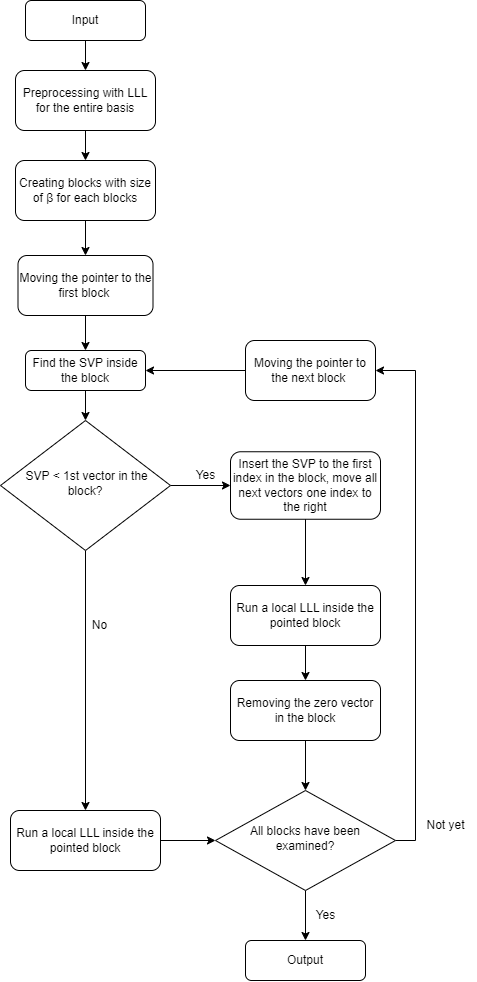
\includegraphics[width=0.7\textwidth]{bkzflowchart.png}
    \caption{The BKZ algorithm}
    \label{BKZ}
\end{figure}
\mbox{}
On the other hand, BKZ (Block Korkine-Zolotarev) .... (Ziyu Zhao et al, 2022)

\subsection{lll-attack-runner}
lll-attack-runner is a Javascript-based interactive web application for running advanced lattice basis reduction algorithms such as LLL and BKZ. It is developed by Zachary Robert Bennett with the latest update was in January 2026. Because we aim to create a Javascript-based interactive web application for visualizing lattice-based cryptographic and cryptanalysis algorithms, in which two of them are LLL and BKZ, we will use lll-attack-runner as the backend for our visualization of the LLL and BKZ algorithms. However, since we want to visualize these two algorithms in an intuitive way which is easier to understand and more practical for cryptography learners, we will develop our own frontend for the visualization.

\subsection{Herramienta de software para la visualización
de la criptografía basada en retículas}
Authored by Jaziel D. Flores Rodríguez and his fellow colleagues, this research paper was aimed to create a visualization tool for post-quantum cryptographic algorithms. The main focus was to graphically visualize mathematical concepts behind these post-quantum cryptographic algorithms, particularly lattice concepts which are the basis of these algorithms. The tool which was developed in this research, successfully visualizes these lattice-based post-quantum cryptographic algorithms within dimensions of 2, 3, 4, and 5. However, the LLL process for dimensions higher than 3 is still not implemented in this tool, and the BKZ algorithm is also not implemented in this tool.
Which is why we will be implementing the LLL process for dimensions higher than 3 in our visualization tool, as well as implementing the BKZ algorithm which is not implemented in this tool.

\section{Architecture}

\subsection{Overview}
\begin{figure}[htbp]
    \centering
    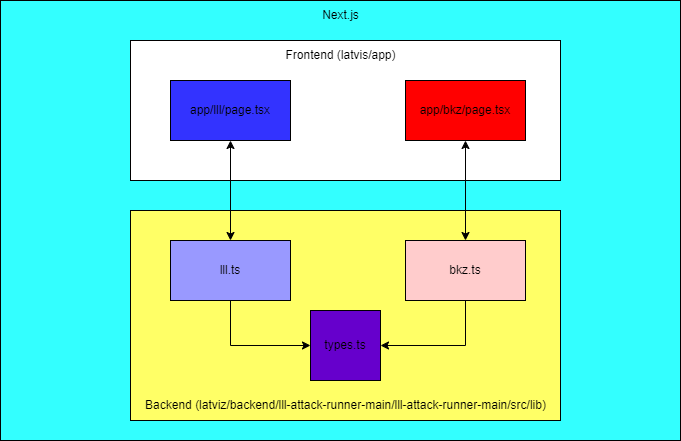
\includegraphics[width=0.7\textwidth]{appstructure.png}
    \caption{Program structure of Latviz's LLL and BKZ visualizers}
    \label{Program diagram structure}
\end{figure}
\mbox{}
Within our source code repository, there is a segregation between the backend and frontend. The role of these backend source codes is to process the inputs inserted from the user through the interface at the frontend. And obviously the role of the frontend section, aside from getting the inputs from the user, is to do the entire visualization jobs. Because the visualization is our main priority, we can say that the frontend section is much more complex compared to the backend one. 

\subsection{Backend}
We're using Zachary Robert Bennett's lll-attack-runner, which is an interactive and Javascript-based lattice-based cryptanalysis solver, as the backend for our visualization of the LLL and BKZ algorithms. We only use three source codes from lll-attack-runner, which are : lll.ts, bkz.ts, and types.ts. The lll.ts, per its filename, does the LLL algorithm process, and the same goes for bkz.ts. Both source codes needs LLLStep interface from types.ts, and for bkz.ts, it also needs LLLRun from lll.ts. 

\subsection{Frontend}
Within the frontend section, in each of BKZ and LLL algorithm modules, each algorithm has its own folder. Which, in each of these folders, there is a single source code written in Typescript, with naming convention of the algorithm name written in lowercase. Each of these source codes are responsible for running the algorithm process which corresponds to their name. Within each of these source codes, we will use imported functions from Zachary Robert Bennett's lll-attack-runner source codes to run the algorithm process.  

We will use Next.js, a React-based framework for building web applications, with the goal to create a user-friendly interface as much as we can for our visualization of the LLL and BKZ algorithms. The user will write their own matrix (or copy-and-paste it from any sources), insert needed values (for example, delta value for both LLL and BKZ algorithm and the block size for BKZ algorithm), and the frontend will pass the values inserted by the user into the backend for the core processing. As what we already explained before in the overview section, the frontend's responsibility is mainly for visualization part.

For the visualization part, we will use D3 for the visualization part, combined with React to create matrices and vectors visualizations. Our secondary objective for the frontend is to create a visualization which have animations for the steps of these algorithms. We believe the animated version of these visualizations can be understand easier by the users. 

\section{Visualization}
\subsection{Vector Representations for Visualizations}
\mbox{}
Vector visualization is a very essential as well an intuitive concept to gain proper understanding of linear algebra concepts (Calderone Dan, 2023). This also includes LLL and BKZ algorithms. And so, for both 2D and 3D visualization panels in each modules of LLL and BKZ, we will depict the vectors extracted from the input (the matrix we inserted) as Euclidean vectors within 2D and 3D Cartesian fields. Here, every single vector is depicted as an arrow that starts from (0,0) as the "anchor", connected with the vectors themselves. Each arrows has different colouring scheme and is unique in terms of value, as every vectors are unique (as they're linearly independent). No vectors would have more than one arrow that represents them (as they all must be linearly independent). %soon will be updated this week also going to fix the bug in LLL and BKZ where two identical vectors are processed and even visualized, something shouldn't be happen (it's likely from the backend part)

\subsection{Output Visualization and Textual Elements for LLL and BKZ}
Visualization of both LLL and BKZ algorithms contains following five visual elements in their output section :

\subsubsection{Graph Panel}
\mbox{}
\begin{figure}[htbp]
    \centering
    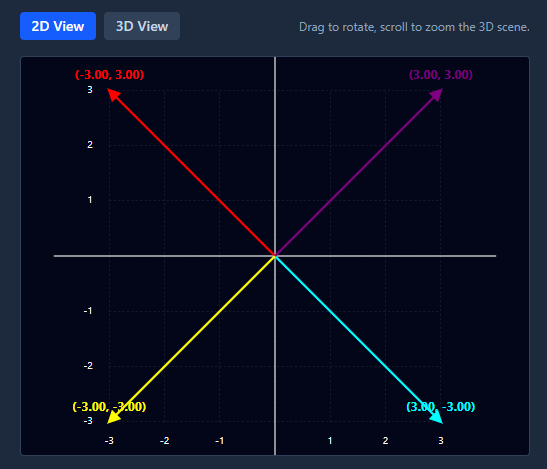
\includegraphics[width=0.7\textwidth]{2Dvisz.png}
    \caption{The 2D visualization}
    \label{2D Visualization}
\end{figure}

\begin{figure}[htbp]
    \centering
    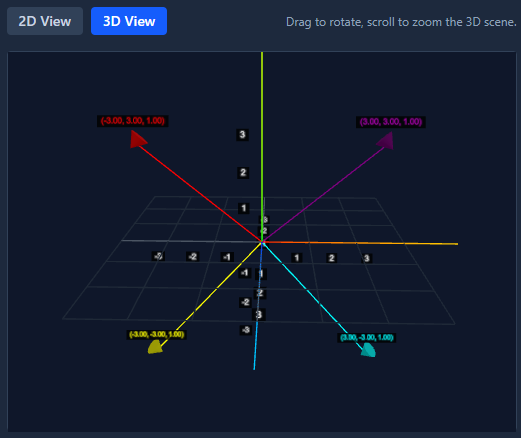
\includegraphics[width=0.7\textwidth]{3Dvisz.png}
    \caption{The 3D visualization}
    \label{3D Visualization}
\end{figure}
\mbox{}
This is the key visual element. Psychologically speaking, human brain is usually better at understanding visual information compared to textual ones (). We design the graph panel in 2D and 3D projections, both in the fashion of the Cartesian coordinate. Each vector arrows represented in this graph panel have different colour, with their vector written in the same colour as their arrow and placed above the tip of their vector arrow. 

\subsubsection{Lovasz Status Panel}
\mbox{}
\begin{figure}[htbp]
    \centering
    
\includegraphics[width=0.7\textwidth]{lovasz.png}
    \caption{The Lovasz Condition is displayed in this panel, whether it's satisfied (shown here) or not}
    \label{Lovasz Status Panel}
\end{figure}

Only shown in the LLL module, the panel shows the user of the Lovasz status of the current basis. If the current basis fulfill the Lovasz condition, it will show the user a green check mark and "Satisfied" text, and if not, a red cross mark and "Not Satisfied" text will be shown to the user. Unlike in its original counterpart, the Lovasz Condition is continously checked throughout the whole LLL process, not just after the basis reduction step, for convenience reasons. %i think i need to add better reasons lol.

\subsubsection{Step and Calculation Details}
\mbox{}
\begin{figure}[htbp]
    \centering
    
\includegraphics[width=0.7\textwidth]{currentstep.png}
    \caption{Current step. Click on the "Show Calculations" for the details}
    \label{Step and Calculation Details}
\end{figure}

This panel will tell the user of the current step (for example, "Basis size reduction"). The user can see the details of the calculation in the step by clicking "Show Calculations" button at the upper right corner of this panel. There are eight types of LLL and BKZ modules : 
\begin{itemize}
\raggedright
\item "Initial Basis". This step is always the first step to be shown after we insert a matrix and clicked "Process Matrix". Right after we clicked the "Process Matrix" button, the program immediately extracted basis vectors from the input. If the "Step" panels shows that the current step is this step, then it means that the program already extracted basis vectors from the input. This step is one of three type of steps who only be shown once, the other two is "Finished" and "Iteration complete" (BKZ-only).
\item 
\item "Gram-Schmidt orthogonalization". Like its algorithm counterpart, the first "Gram-Schmidt orthogonalization" step would be shown as the second step in a matrix process. In this step, the program performs Gram-Schmidt orthogonalization (GSO) for all vectors from the input, produces the initial orthogonalized $\mathbf{v}_k^*$ and their corresponding projection coefficients $\mu_{k,j}$, with $1 \le j < k \le n$. This step also would be executed should a basis doesn't satisfies the Lovasz Condition (in this program, depicted in the form of a panel on its own). 
\item
\item "Basis reduction". It represents the basis reduction step from the original algorithm, in which a vector that is currently examined (started from the second vector in the basis from the input), having been orthogonalized globally during the Gram-Schmidt orthogonalization step previously together with all other vectors in the basis from the input, is being subtracted by the previous vector (), in order to shorten the currently examined vector. This step also would be executed should a basis doesn't satisfies the Lovasz Condition. 
\item 
\item "Basis swap". This step is only executed and shown if during the "real" Lovasz Condition checking (which is executed after the basis reduction step, just like in the original algorithm), the Lovasz Condition isn't satisfied. In this step, like its namesake, the vector which are currently examined, has its index swapped with the previous vector. 
\item 
\item "Start LLL Process $\#n$". Only in the BKZ module, when this step is shown, it means that the LLL process in the current block is being executed (in the n-th iteration).
\item 
\item "Complete LLL Process $\#n$". Also only in the BKZ module, when this step is shown, it means that the LLL process in the current block is has been completed (in the n-th iteration).
\item 
\item "Iteration Complete". Like two previous steps, this is also a BKZ module-only type of step. Like its namesake, if this step is shown, then an iteration is stated to be completed, and unless it's the final iteration, the next iteration begins immediately.
\item  
\item "Finished". This step is in both LLL and BKZ modules. If this state is shown, then the program (LLL or BKZ, depends on what the module we currently use) terminates. In the context of their respective algorithms, if this step is reached, for LLL, all vectors has been examined and the Lovasz Condition is satisfied for the basis from the input, which in the other words, the basis has been successfully shortened and orthogonalized in accordance to the $\delta$-value. For BKZ, all blocks has been examined (the Lovasz Condition is checked inside each block as part of the local LLL process). 
\end{itemize}

\subsubsection{Current Basis Panel}
\mbox{}
\begin{figure}[htbp]
    \centering
    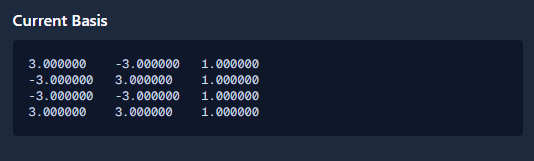
\includegraphics[width=0.7\textwidth]{currentbasis.png}
    \caption{The current basis as with the current step}
    \label{Current Basis Panel}
\end{figure}
Like its namesake, this panel's sole function is to show the user the current basis. 

\subsubsection{Shortest Vector Panel (BKZ only)}
\mbox{}
\begin{figure}[htbp]
    \centering
    
\includegraphics[width=0.7\textwidth]{svpres.png}
    \caption{The SVP we gained, which only shown in the final step of the BKZ process}
    \label{SVP}
\end{figure}

Only for BKZ algorithm, this panel's sole function is to inform the user the shortest vectors found in the current basis. Only shown in the last step.

\subsection{Visualization of the LLL Algorithm}
First, we have the LLL algorithm. The input panel for this algorithm has matrix and delta value insertion fields, and located in the left half of the page. After the user inserted matrix and delta value properly, and clicked "Process Matrix" button, user can see the "Initial Matrix" as well "Initial Basis" panels below the input panel. To the right half of the page, there is the output section, contains four of five visual and textual information panels, without Shortest Vector Panel. 

User can click "Back" and "Next" button in the upper part of the output section to see the previous and next steps of the LLL algorithm process. All visual and textual information panels in the output section are subjects of change according to the current step of the LLL algorithm process. 

\subsection{Visualization of the BKZ Algorithm}
Next, we have the BKZ algorithm, which is one of the more powerful lattice reduction algorithm. Because theoritically this algorithm could be comprised of multiple LLL processes, we design the output section to show the user the number of LLL processes as well an additional information called "Current Process", which provides the user of the steps that is unique to BKZ algorithm, which are the current number of the LLL process and SVP enumeration. 

The only differences with LLL page is in the input panel, which has an additional, mandatory field for the block size, and in the output section, in which has Shortest Vector panel. Moreover, in the upper part of the output section, we place four additional information, which are "Block Size", "Delta", "Total LLL Processes", and "Current Process". Out of all of these additional information, only "Current Process" isn't static. 

Aside from additional panels and input field, the rest of the visualization and basically mechanism of the output's UI is the same as the LLL ones. 

\section{Result}
Please note that the first paragraph of a section or subsection is
not indented. The first paragraph that follows a table, figure,
equation etc. does not need an indent, either.

Subsequent paragraphs, however, are indented.

\subsection{LLL Visualization} 
insert ss of the web here with similar matrix to bkz
\subsection{BKZ Visualization}
insert ss of the web here with similar matrix to lll

\section{Evaluation}

\section{Conclusion}

\begin{thebibliography}{8}
\bibitem{ref_1}
Ziyu Zhao, Jintai Ding. (2022). Practical Improvements on BKZ Algorithm. National Institute of Standards and Technology \url{https://csrc.nist.gov/csrc/media/Events/2022/fourth-pqc-standardization-conference/documents/papers/practical-improvements-on-bkz-algorithm-pqc2022.pdf}

\bibitem{ref_2}
Mayer, RE. (2001). Multimedia Learning. Cambridge University Press.

\bibitem{ref_3}
Christopher D. Hundhausen, Sarah A. Douglas, John Stasko. (2002). A Meta-Study of Algorithm Visualization Effectiveness. Journal of Visual Languages and Computing, 13(3), 259-290. 

\bibitem{ref_4}
A.Cihan Konyaliouglu, Ahmet Isik, Abdullah Kaplan, Seyfullah Hizarci, Merve Durkaya. (2011). Visualization approach in teaching process of linear algebra. Procedia Social and Behavioral Sciences 15 (2011) 4040-4044. 

\bibitem{ref_5}
Wang Yunfei, Jin Xin, Liu Junyu. (2025). Learning with errors may remain hard against quantum holographic attacks arXiv:2509.22833

\bibitem{ref_6}
Silverman, Joseph H. (2020). An Introduction to Lattices, Lattice Reduction, and Lattice-Based Cryptography. IAS/Park City Mathematics Series Graduate Summer School Lecture Notes. 

\bibitem{ref_7}
Meyer Alexander. (2024). Post-Quantum Cryptography: An Analysis of Code-Based and Lattice-Based Cryptosystem. arXiv:2505.08791. 

\bibitem{ref_8}
Calderone, Dan. (2023). Vector Visualizations. Github.

\bibitem{ref_9}
Author, F., Author, S., Author, T.: Book title. 2nd edn. Publisher,
Location (1999)

\bibitem{ref_proc1}
Author, A.-B.: Contribution title. In: 9th International Proceedings
on Proceedings, pp. 1--2. Publisher, Location (2010)

\bibitem{ref_url1}
LNCS Homepage, \url{http://www.springer.com/lncs}, last accessed 2023/10/25
\end{thebibliography}

\begin{equation}
x + y = z
\end{equation}
Please try to avoid rasterized images for line-art diagrams and
schemas. Whenever possible, use vector graphics instead

%
% the environments 'definition', 'lemma', 'proposition', 'corollary',
% 'remark', and 'example' are defined in the LLNCS documentclass as well.

%
% ---- Bibliography ----
%
% BibTeX users should specify bibliography style 'splncs04'.
% References will then be sorted and formatted in the correct style.
%
% \bibliographystyle{splncs04}
% \bibliography{mybibliography}
%
\end{document}
